\documentclass[12pt]{article}

\usepackage[margin=1in]{geometry}
\usepackage{amsmath, amssymb}
\usepackage{graphicx}
\usepackage{booktabs}
\usepackage{array}
\usepackage{caption}
\usepackage{subcaption}
\usepackage{hyperref}
\usepackage{setspace}
\usepackage{float}
\usepackage[table]{xcolor}
\usepackage{microtype}
\usepackage{enumitem}
\usepackage{natbib}

\hypersetup{
    colorlinks=true,
    linkcolor=blue!60!black,
    citecolor=blue!60!black,
    urlcolor=blue!60!black
}

\onehalfspacing

% -----------------------------------------------------------------------
% TITLE PAGE
% -----------------------------------------------------------------------

\title{\textbf{Selective Prediction and the Persistence Illusion:\\
A Diagnostic Decomposition of VIX Regime Classification}}

\author{
    Akshat Gupta\textsuperscript{1} \and
    Jianguo Liu\textsuperscript{2,*}
}

\date{}

\begin{document}

\maketitle

\noindent\textsuperscript{1} Texas Academy of Mathematics and Science, University of North Texas,
Denton, TX 76203, USA; akshatguptaakshatgupta@gmail.com; ORCID: 0009-0003-7993-1640\\
\textsuperscript{2} Department of Mathematics, University of North Texas, Denton, TX 76203, USA\\
\textsuperscript{*} Correspondence: jianguo.liu@unt.edu

\vspace{1em}
\noindent\textbf{Abstract:}
Confidence-based selective prediction systems for financial regime classification can achieve
apparent accuracy exceeding 90\% while providing no genuine predictive skill beyond naive
persistence. We demonstrate this through a systematic diagnostic study of VIX regime
classification across 5,000 trading days (July 2006--May 2026). A six-component evaluation
protocol---comprising coverage-matched baseline comparison, persistence quantification,
regime-transition accuracy audit, SHAP feature attribution, LSTM comparison, and abstention
confound testing---reveals that a three-feature HAR-style logistic regression matches or exceeds
a 36-feature Random Forest at four of five prediction horizons under moving-block bootstrap
testing. A coverage-matched persistence rule makes identical predictions to the Random Forest on
every jointly covered day at horizons $N \geq 10$ (McNemar $b = c = 0$), confirming that any
accuracy gap is attributable to coverage composition rather than multi-feature predictive skill.
The confidence filter achieves 0\% accuracy on calm-to-high volatility transition days at all
horizons; explicit cost-weighting up to $20{\times}$ does not improve this, establishing an
informational ceiling rather than an objective-function deficiency. These results replicate on
S\&P 500 trend regimes, establishing the persistence illusion as a structural property of
selective prediction on serially correlated labels. The diagnostic protocol is modular and
directly applicable to any selective prediction system on autocorrelated outcomes.

\vspace{0.5em}
\noindent\textbf{Keywords:} VIX regime classification; selective prediction; persistence illusion;
machine learning; Random Forest; volatility forecasting; autocorrelation artifact

\vspace{0.5em}
\noindent\textbf{JEL Classification:} C53; C63; G10; G17; C12

% -----------------------------------------------------------------------
\section{Introduction}
% -----------------------------------------------------------------------

Volatility is one of the most important dimensions of financial market risk. The CBOE Volatility
Index (VIX), often described as the market's ``fear gauge,'' summarizes option-implied
expectations of S\&P 500 volatility over the next 30 days and is widely used by investors, risk
managers, and policymakers to monitor uncertainty in equity markets \citep{whaley2009}. When VIX
rises above 20---a level widely adopted as a practical divide between normal and elevated-fear
environments \citep{whaley2009}---markets are generally considered to be in a high-volatility
regime characterized by elevated fear, widening credit spreads, and increased probability of large
equity drawdowns. Episodes such as the COVID-19 crash of March 2020 and the Japan carry-trade
unwind of August 2024 illustrate the costs of failing to anticipate these regime transitions.

Despite its importance, VIX regime prediction is a difficult problem. Volatility is noisy,
mean-reverting, and driven by a complex mixture of market sentiment, equity conditions, interest
rates, and sudden exogenous shocks. Classical approaches such as GARCH-family models
\citep{bollerslev1986} and Markov-switching frameworks \citep{hamilton1989} have provided
important foundations, but often assume specific parametric structures that may not hold in
practice. Machine learning methods offer flexibility in modeling nonlinear interactions across
large feature sets, but introduce their own challenges: temporal leakage, calibration, and---
critically for regime classification---the difficulty of distinguishing genuine predictive skill
from the strong autocorrelation inherent in VIX.

The selective prediction literature---which studies classifiers that may abstain from uncertain
predictions \citep{chow1970, bartlett2008, geifman2017}---offers a principled solution: reserve
predictions for high-confidence cases, trading coverage for reliability on predicted days. On
autocorrelated label sequences such as VIX regimes, however, selective prediction can manufacture
the appearance of skill by preferentially covering easy regime-stable days.

This paper develops a confidence-based selective prediction framework for VIX regime
classification and uses it as a lens to examine where accuracy gains come from and what they are
worth. Two ensemble classifiers---Random Forest (RF) and Histogram Gradient Boosting (HGB)---are
trained on 36 features and abstain when calibrated probability is close to 0.5. The headline
accuracy figures (90--93\% for RF at $\tau = 0.25$) are striking, but a systematic decomposition
reveals that they constitute a diagnostic, not an achievement.

The main findings are as follows. First, a HAR-style logistic regression using only three
features (current VIX level, 5-day VIX mean, 20-day VIX mean) matches or exceeds the full
36-feature RF in point estimate at four of five horizons at matched coverage; the HAR-minus-RF
gap at $N = 10$ is $+1.1$ percentage points (pp; HAR leads), with bootstrap 95\% CI
$[-1.08, +4.18]$, so the advantage is a pattern, not a confirmed result. Second, a
coverage-matched naive persistence rule closely tracks RF performance at all horizons; a McNemar
test on jointly covered days finds $b = c = 0$ at $N \geq 10$: RF and persistence make identical
predictions on every shared day. Third, the confidence filter covers 87\% of calm-persisting days
at $N = 5$ but yields 0\% accuracy on every calm$\to$high transition it covers; explicit
cost-weighting up to $20{\times}$ does not overcome this. Fourth, at $N = 25$, balanced accuracy
collapses to 50\% for both RF and HGB. Fifth, persistence at matched coverage dominates RF
selective prediction on cost-weighted utility whenever false negatives are more costly than false
alarms ($C \geq 5$) at $N = 10$.

The remainder of the paper is organized as follows. Section~\ref{sec:related} reviews related
work. Section~\ref{sec:data} describes the data. Section~\ref{sec:methodology} presents the
methodology. Section~\ref{sec:results} reports empirical results. Section~\ref{sec:replication}
replicates the diagnostic on S\&P 500 trend regimes. Section~\ref{sec:conclusion} concludes.

% -----------------------------------------------------------------------
\section{Related Work}
\label{sec:related}
% -----------------------------------------------------------------------

\subsection{Volatility Forecasting and Regime Modeling}

The modeling of financial volatility has a long history in econometrics.
\citet{bollerslev1986} introduced the GARCH model, which captures the tendency of volatility
to cluster over time by modeling conditional variance as a function of past squared residuals.
GARCH-family models have since been extended in numerous directions and remain a standard
benchmark for volatility forecasting. \citet{hamilton1989} introduced Markov-switching models,
in which a time series is assumed to switch between discrete latent states according to a Markov
chain. This framework provides a natural model for regime transitions and has been widely applied
to financial and macroeconomic time series. \citet{guidolin2007} extended regime-switching ideas
to multivariate portfolio allocation settings, demonstrating that regime-dependent models can
outperform single-state specifications in out-of-sample asset allocation.

A complementary strand of work focuses on realized volatility constructed from high-frequency
intraday returns. \citet{corsi2009} proposed the Heterogeneous Autoregressive (HAR) model, which
captures the long-memory properties of realized volatility through a simple additive structure of
daily, weekly, and monthly volatility components. The HAR model has become a standard benchmark
for realized volatility forecasting, and its strong performance motivates including a HAR-style
logistic regression as a baseline in this paper.

In the VIX-specific literature, \citet{whaley2009} documented the VIX's role as a fear indicator
and its asymmetric behavior in market downturns. \citet{fernandes2014} studied the predictability
of VIX using a variety of econometric models and found that simple autoregressive specifications
perform competitively against more complex alternatives. This paper replicates and extends that
finding: simple HAR-style models are competitive with 36-feature ensemble classifiers on the
binary regime classification task.

\subsection{Machine Learning for Financial Prediction}

Machine learning methods have increasingly been applied to financial forecasting. Ensemble methods
such as Random Forests \citep{breiman2001} and Gradient Boosting are particularly well-suited to
financial prediction because they can model nonlinear interactions among large feature sets without
requiring distributional assumptions.

A key methodological challenge in applying machine learning to financial data is avoiding data
leakage and respecting the temporal ordering of observations. This paper addresses this by using
chronological train/test splitting, \texttt{TimeSeriesSplit} cross-validation during calibration,
and walk-forward validation as a robustness check---consistent with best practices in applied
financial machine learning.

\subsection{Selective Prediction and the Reject Option}

The reject option in classification allows a model to abstain from making a prediction when its
confidence is insufficient. \citet{chow1970} first formalized the optimal reject option.
\citet{bartlett2008} studied classification with a reject option using hinge loss and established
theoretical generalization bounds. \citet{geifman2017} demonstrated that selective prediction
can substantially improve reliability in modern deep learning settings.

In financial applications, the reject option is particularly natural. A risk model that provides
no signal on ambiguous days is often more useful than one that forces a low-confidence prediction.
However, on autocorrelated series such as VIX regimes, abstention can manufacture accuracy without
genuine predictive skill---the central diagnostic this paper examines.

% -----------------------------------------------------------------------
\section{Data}
\label{sec:data}
% -----------------------------------------------------------------------

\subsection{Market Data}

Daily price data are obtained from Yahoo Finance for eight market series: the CBOE Volatility
Index (VIX), the 3-month VIX term structure index (VIX3M), the CBOE 9-Day Volatility Index
(VIX9D), the S\&P 500 Index, gold futures (GC=F), the 10-Year Treasury Yield (TNX), the U.S.\
Dollar Index (DXY), and the CBOE SKEW Index. VIX9D is downloaded to keep the raw data complete
but is not used as a model feature. Although raw VIX data is available from January 1990, VIX3M
data begins in July 2006; because VIX3M anchors the term spread feature, the effective sample
starts on July 17, 2006.

\subsection{Macroeconomic Data}

Two macroeconomic variables are obtained from the Federal Reserve Economic Data (FRED) API: the
Federal Funds Rate and the 10-Year minus 2-Year Treasury yield curve spread (T10Y2Y). The Federal
Funds Rate target is forward-filled to daily frequency by holding the prevailing rate constant
between FOMC meeting dates.

\subsection{Label Construction}

The prediction task is binary regime classification. For a prediction horizon $N$, the label is:
\begin{equation}
    \text{LABEL}_{N,t} = \begin{cases} 1 & \text{if } \text{VIX}_{t+N} \geq 20 \\ 0 & \text{if } \text{VIX}_{t+N} < 20 \end{cases}
    \label{eq:label}
\end{equation}

The label is forward-shifted $N$ days to ensure that all features are observed at time $t$ and
the outcome is measured at time $t + N$, eliminating lookahead bias. Horizons
$N \in \{5, 10, 15, 20, 25\}$ trading days are evaluated.

A \emph{sustained-high} label is also constructed:
\begin{equation}
    \text{SUSTAINED\_LABEL}_{N,t} = \begin{cases} 1 & \text{if } \text{VIX}_{t+k} \geq 20 \;\text{for all}\; k \in \{1, \ldots, N\} \\ 0 & \text{otherwise} \end{cases}
    \label{eq:sustained}
\end{equation}

\subsection{Class Distribution and Train/Test Split}

The full feature dataset covers 5,000 trading days from July 17, 2006 to May 29, 2026. Data
are split chronologically, with the first 80\% used for training (2006--2022) and the remaining
20\% for testing (2022--2026), preserving strict temporal ordering.

\begin{table}[H]
\centering
\caption{Class distribution (fraction of days with VIX $\geq$ 20) by dataset split.}
\label{tab:class}
\begin{tabular}{lccc}
\toprule
Split & VIX $\geq$ 20 & VIX $<$ 20 & Majority-class baseline \\
\midrule
Training (2006--2022) & 36.7\% & 63.3\% & 63.3\% \\
Test (2022--2026)     & 29.8\% & 70.2\% & 70.2\% \\
\bottomrule
\end{tabular}
\end{table}

High-volatility days are substantially less common in the test period ($\approx$30\%) than in
training ($\approx$37\%), reflecting that the training window encompasses several high-volatility
crises---the 2008--09 financial collapse, the 2011 eurozone episode, and the COVID-19 crash---
whereas the test window is dominated by the post-bear-market recovery despite the elevated
volatility of the first half of 2022.

% -----------------------------------------------------------------------
\section{Methodology}
\label{sec:methodology}
% -----------------------------------------------------------------------

\subsection{Feature Engineering}

The model uses 36 engineered features grouped into five categories. All features are computed
using only information available at or before the prediction date $t$.

\textbf{VIX technical indicators} (13 features): 10-day and 20-day simple moving averages
(SMA10, SMA20); 10-day and 20-day momentum; 10-day and 20-day rate of change; Bollinger Band
standard deviation, upper and lower bands, and position within the band; 14-day RSI;
moving-average cross (SMA10 $-$ SMA20); and VIX term spread (VIX3M $-$ VIX).

\textbf{SKEW features} (3 features): SKEW level, 5-day change, and 20-day change.

\textbf{S\&P 500 features} (7 features): 1-day, 5-day, and 20-day returns; 10-day and 20-day
price momentum; 20-day realized volatility; and 252-day maximum drawdown.

\textbf{Cross-asset features} (9 features): Gold 1-day, 5-day, and 20-day returns; 10-Year
Treasury Yield 1-day, 5-day, and 20-day changes; DXY 1-day, 5-day, and 20-day returns.

\textbf{Macroeconomic features} (4 features): Federal Funds Rate 1-month and 3-month changes;
yield curve spread 1-month and 3-month changes.

The complete feature list appears in Appendix~\ref{app:features}.

\subsection{Models and Training Pipeline}

Two ensemble classifiers are evaluated: Random Forest (RF) and Histogram Gradient Boosting
(HGB), both implemented via scikit-learn. Both use a single fixed specification: RF with
\texttt{n\_estimators=200}, \texttt{max\_depth=10}, \texttt{min\_samples\_leaf=5};
HGB with \texttt{max\_iter=200}, \texttt{max\_depth=5}, \texttt{learning\_rate=0.1}.
All seeds set to \texttt{random\_state=42}. Using one specification eliminates pipeline inconsistencies
and provides a fair comparison across tables. All features are standardized using
\texttt{StandardScaler} fit on the training set and applied to the test set.

\subsection{Probability Calibration}

The selective prediction rule requires well-calibrated probability estimates. We apply isotonic
regression calibration using \texttt{CalibratedClassifierCV} with 5-fold
\texttt{TimeSeriesSplit} cross-validation on the full training set. The calibrated probability
at time $t$ is denoted $\hat{p}_t$, representing the estimated probability that VIX will be in a
high-volatility regime at $t + N$.

\subsection{Confidence-Based Selective Prediction}

The selective classifier makes a prediction only when $\hat{p}_t$ is sufficiently far from 0.5.
For confidence threshold $\tau \in (0, 0.5)$, the prediction rule is:
\begin{equation}
    \hat{y}_t = \begin{cases}
        1 & \text{if } \hat{p}_t > 0.5 + \tau \\
        0 & \text{if } \hat{p}_t < 0.5 - \tau \\
        \text{abstain} & \text{if } 0.5 - \tau \leq \hat{p}_t \leq 0.5 + \tau
    \end{cases}
    \label{eq:selective}
\end{equation}

Accuracy is evaluated only on days where the model makes a prediction. Coverage is defined as
the fraction of test days on which a prediction is made. The primary threshold is $\tau = 0.25$.

% -----------------------------------------------------------------------
\section{Results}
\label{sec:results}
% -----------------------------------------------------------------------

\subsection{Main Accuracy Results}
\label{sec:main}

Table~\ref{tab:main} reports baseline and selective accuracy, coverage, and balanced accuracy
on covered days at $\tau = 0.25$.

\begin{table}[H]
\centering
\caption{Baseline and selective ($\tau = 0.25$) accuracy, coverage, and balanced accuracy on
covered days. Gain = selective minus baseline in percentage points (pp).}
\label{tab:main}
\resizebox{\textwidth}{!}{%
\begin{tabular}{cccccccccc}
\toprule
$N$ & RF Base & RF Sel & RF Gain & RF Cov & RF BalAcc & HGB Sel & HGB Gain & HGB Cov & HGB BalAcc \\
\midrule
5  & 83.4\% & 91.9\% & $+$8.5 pp & 76.3\% & 88.4\% & 92.1\% & $+$8.9 pp & 71.1\% & 88.2\% \\
10 & 79.5\% & 90.0\% & $+$10.5 pp & 60.1\% & 84.8\% & 92.2\% & $+$13.6 pp & 63.1\% & 86.1\% \\
15 & 76.2\% & 90.0\% & $+$13.8 pp & 51.3\% & 83.9\% & 92.2\% & $+$21.3 pp & 36.0\% & 89.5\% \\
20 & 76.8\% & 92.7\% & $+$15.9 pp & 31.7\% & 79.1\% & 94.8\% & $+$22.2 pp & 26.8\% & 84.1\% \\
25 & 73.4\% & 90.3\% & $+$16.9 pp & 26.9\% & \textbf{50.0\%} & 92.7\% & $+$26.5 pp & 19.2\% & \textbf{50.0\%} \\
\bottomrule
\end{tabular}}
\end{table}

\begin{table}[H]
\centering
\caption{Extended metrics on covered days for Random Forest ($\tau = 0.25$). At $N = 25$,
precision and recall are both 0\% and balanced accuracy equals 50\%, confirming the model
exclusively predicts the calm class at this horizon.}
\label{tab:extended}
\begin{tabular}{cccccc}
\toprule
$N$ & Selective Acc & Precision & Recall & F1 & Balanced Acc \\
\midrule
5  & 91.9\% & 86.5\% & 81.2\% & 83.8\% & 88.4\% \\
10 & 90.0\% & 86.8\% & 73.8\% & 79.7\% & 84.8\% \\
15 & 90.0\% & 89.8\% & 70.8\% & 79.2\% & 83.9\% \\
20 & 92.7\% & 100.0\% & 58.2\% & 73.6\% & 79.1\% \\
25 & 90.3\% & 0.0\% & 0.0\% & 0.0\% & \textbf{50.0\%} \\
\bottomrule
\end{tabular}
\end{table}

\begin{figure}[H]
    \centering
    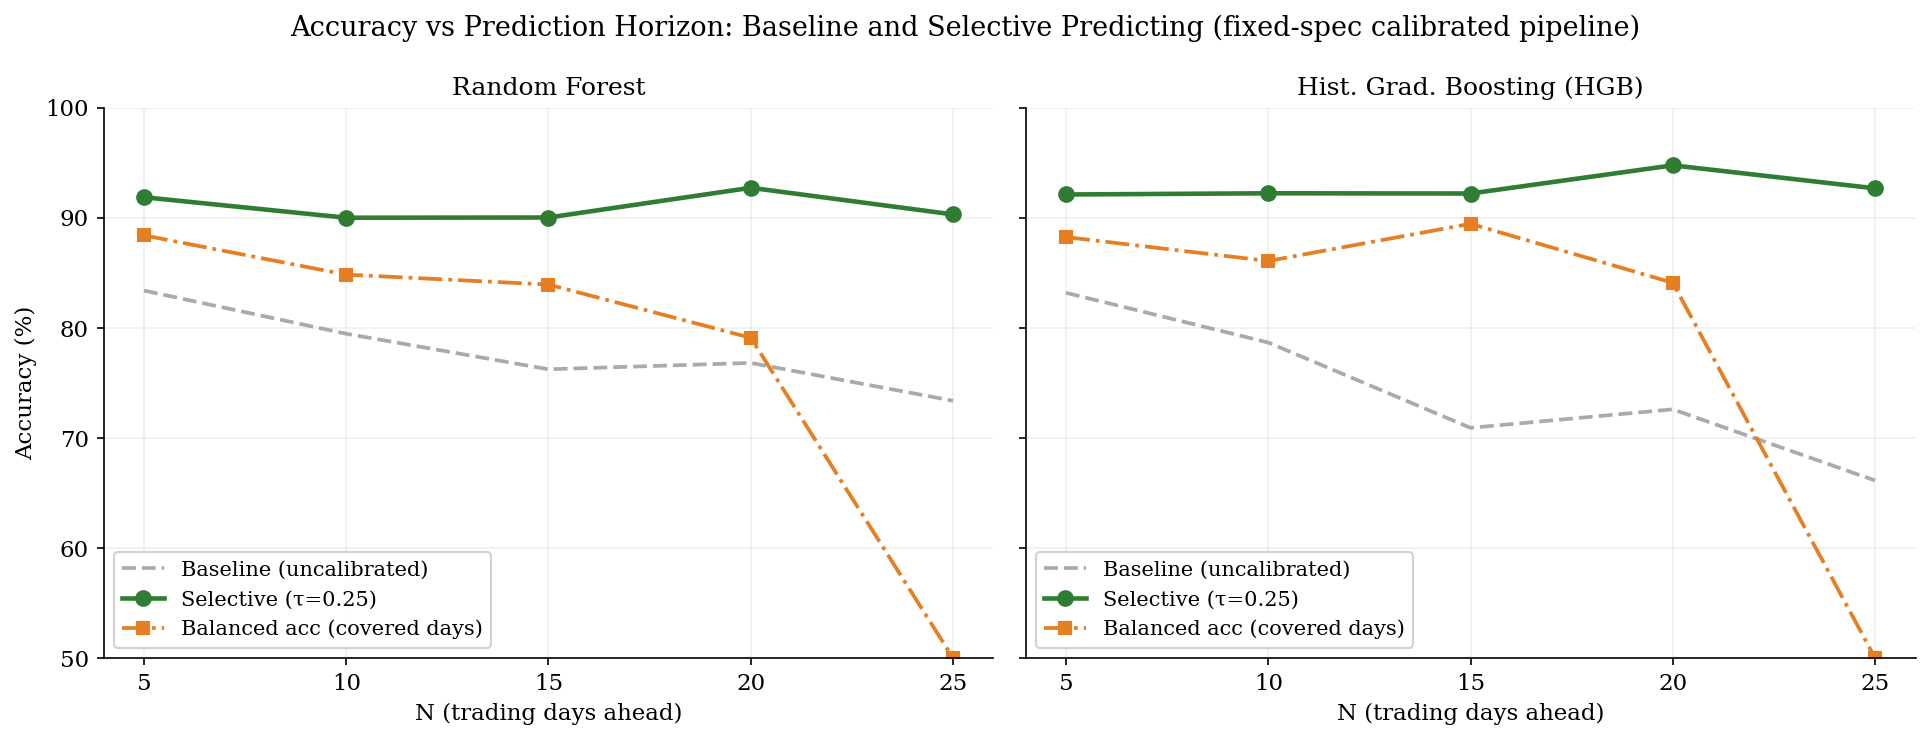
\includegraphics[width=0.85\textwidth]{tuned_model_comparison.png}
    \caption{Baseline, selective accuracy, and balanced accuracy across prediction horizons for
    Random Forest (left) and HGB (right). At $N = 25$, balanced accuracy equals 50\%, confirming
    a coin-flip result despite 90\% selective accuracy.}
    \label{fig:main}
\end{figure}

Selective prediction improves accuracy for both models at every horizon. However, the balanced
accuracy columns reveal the underlying artifact: RF balanced accuracy declines monotonically
from 88.4\% at $N = 5$ to 50.0\% at $N = 25$. This collapse confirms that the model
exclusively predicts calm outcomes at the longest horizon, and the nominal 90\% selective
accuracy reflects the 70\% base rate of calm days, not predictive skill.

\subsection{Threshold Sensitivity}

\begin{table}[H]
\centering
\caption{Random Forest selective accuracy and coverage as a function of confidence threshold
$\tau$.}
\label{tab:threshold}
\begin{tabular}{ccccc}
\toprule
$\tau$ & RF $N{=}5$ Acc & $N{=}5$ Cov & RF $N{=}10$ Acc & $N{=}10$ Cov \\
\midrule
0.10 & 86.5\% & 91.0\% & 83.3\% & 90.5\% \\
0.15 & 88.3\% & 85.1\% & 84.7\% & 85.9\% \\
0.20 & 89.0\% & 82.9\% & 86.6\% & 78.5\% \\
0.25 & 91.9\% & 76.3\% & 90.0\% & 60.1\% \\
0.30 & 92.3\% & 73.6\% & 91.8\% & 53.6\% \\
0.35 & 95.0\% & 67.1\% & 95.1\% & 36.5\% \\
0.40 & 97.4\% & 49.0\% & 97.4\% & 15.3\% \\
\bottomrule
\end{tabular}
\end{table}

Accuracy increases monotonically with $\tau$ across all horizons, confirming that the calibrated
probability is a reliable ranking signal. However, as Section~\ref{sec:transitions} shows,
increasing $\tau$ does not improve coverage of transition days---it makes confident wrong
predictions on calm$\to$high days even more selective.

\subsection{Robustness Across VIX Thresholds}

\begin{table}[H]
\centering
\caption{Random Forest accuracy gain (selective vs.\ baseline) by VIX regime threshold at
$\tau = 0.25$.}
\label{tab:robust}
\begin{tabular}{cccc}
\toprule
$N$ & VIX $\geq$ 18 & VIX $\geq$ 20 & VIX $\geq$ 22 \\
\midrule
5  & $+$5.4 pp  & $+$8.5 pp  & $+$7.5 pp  \\
10 & $+$11.3 pp & $+$10.5 pp & $+$10.3 pp \\
15 & $+$14.8 pp & $+$13.8 pp & $+$7.9 pp  \\
20 & $+$22.3 pp & $+$15.9 pp & $+$9.1 pp  \\
25 & $-$14.8 pp & $+$16.9 pp & $+$8.3 pp  \\
\bottomrule
\end{tabular}
\end{table}

The advantage of selective prediction holds across VIX thresholds of 18, 20, and 22 at
$N \leq 20$. The exception is RF at $N = 25$, VIX $\geq$ 18, which shows a gain of $-14.8$ pp,
consistent with the degenerate behavior documented in Table~\ref{tab:extended}.

\subsection{Sustained Regime Labels}
\label{sec:sustained}

\begin{table}[H]
\centering
\caption{Random Forest selective accuracy for instantaneous and sustained regime labels at
$\tau = 0.25$.}
\label{tab:sustained}
\begin{tabular}{ccc}
\toprule
$N$ & Instantaneous & Sustained \\
\midrule
5  & 91.9\% & 94.0\% \\
10 & 90.0\% & 93.8\% \\
15 & 90.0\% & 93.8\% \\
20 & 92.7\% & 94.3\% \\
25 & 90.3\% & 89.9\% \\
\bottomrule
\end{tabular}
\end{table}

Sustained regime labels are consistently easier to predict than instantaneous labels at
$N \leq 20$, reflecting that persistent high-volatility episodes are preceded by stronger
signals across multiple features.

\subsection{Comparison to Naive Baselines}
\label{sec:baselines}

A critical question is whether the RF selective accuracy reflects genuine multi-feature ML skill
or simply VIX autocorrelation. To answer this, we construct four coverage-matched baselines
evaluated on the same test set.

The \textbf{persistence baseline} predicts $\text{VIX}_{t+N} \geq 20$ if and only if
$\text{VIX}_t \geq 20$, and abstains when $|\text{VIX}_t - 20| < c$ for a constant $c$ chosen
to match the RF's coverage. The \textbf{LR (VIX only) baseline} applies the full calibration
pipeline to a single feature (current VIX level). The \textbf{HAR-style logistic regression}
uses three features motivated by the HAR model \citep{corsi2009}: current VIX ($\text{VIX}_D$),
5-day VIX mean ($\text{VIX}_W$), and 20-day VIX mean ($\text{VIX}_M$). The
\textbf{Markov-chain baseline} estimates the 1-step transition probability matrix from training
data and raises it to the $N$th power.

\begin{table}[H]
\centering
\caption{RF selective accuracy vs.\ naive baselines at matched coverage ($\tau = 0.25$).
Bolded values indicate where a baseline exceeds the RF selective accuracy.}
\label{tab:baselines}
\begin{tabular}{cccccccc}
\toprule
$N$ & Coverage & Persistence & LR (VIX) & \textbf{HAR-LR} & Markov & RF Sel & RF$-$Persist \\
\midrule
5  & 76.3\% & 91.6\% & 91.8\% & 91.6\% & 83.7\% & 91.9\% & $+$0.3 pp \\
10 & 60.1\% & 88.1\% & 87.6\% & \textbf{91.1\%} & 85.3\% & 90.0\% & $+$1.9 pp \\
15 & 51.3\% & 87.9\% & 88.4\% & \textbf{90.2\%} & 84.8\% & 90.0\% & $+$2.1 pp \\
20 & 31.7\% & 90.5\% & 87.9\% & \textbf{94.2\%} & 84.5\% & 92.7\% & $+$2.3 pp \\
25 & 26.9\% & 83.8\% & 86.8\% & \textbf{92.0\%} & 82.9\% & 90.3\% & $+$6.5 pp \\
\bottomrule
\end{tabular}
\end{table}

\begin{figure}[H]
    \centering
    
\includegraphics[width=0.85\textwidth]{persistence_baseline.png}
    \caption{Left: RF selective vs.\ naive baseline accuracy at matched coverage across horizons.
    Right: RF vs.\ persistence gap with 95\% moving-block bootstrap CI. No bar is statistically
    significant at 5\%.}
    \label{fig:baselines}
\end{figure}

Table~\ref{tab:baselines} delivers the paper's sharpest negative result. The HAR-style logistic
regression---using only three VIX-related features---matches or exceeds the full 36-feature RF
in point estimate at four of five horizons ($N = 10$, 15, 20, and 25). A moving-block bootstrap
on the HAR-minus-RF gap at $N = 10$ (HAR leads by $+1.1$ pp) yields 95\% CI $[-1.08, +4.18]$;
the corresponding RF-minus-persistence bootstrap gives CI $[-1.11, +4.17]$. Neither gap is
statistically confirmed. The 33 additional features contribute negligibly beyond the
three-variable VIX autoregressive structure.

\subsection{Persistence Quantification}
\label{sec:persist_quant}

For each horizon $N$, we compute the empirical transition probabilities
$\Pr(\text{VIX}_{t+N} \geq 20 \mid \text{VIX}_t \geq 20)$ and
$\Pr(\text{VIX}_{t+N} \geq 20 \mid \text{VIX}_t < 20)$, and classify each correct RF covered
prediction as either a same-regime or regime-change call.

\begin{table}[H]
\centering
\caption{Empirical VIX transition probabilities and decomposition of RF correct covered
predictions. P(H$\mid$H) = P(VIX$_{t+N} \geq 20 \mid$ VIX$_t \geq 20$); P(H$\mid$C) =
P(VIX$_{t+N} \geq 20 \mid$ VIX$_t < 20$). Same-regime \% = fraction of correct RF covered
predictions that match the regime at $t$.}
\label{tab:persist_quant}
\begin{tabular}{cccccc}
\toprule
$N$ & P(H$\mid$H) & P(H$\mid$C) & Persist.\ ratio & RF cov.\ acc & Same-regime \% \\
\midrule
5  & 84.2\% &  8.6\% & 9.8$\times$ & 91.9\% & 99.0\% \\
10 & 79.5\% & 11.2\% & 7.1$\times$ & 90.0\% & 99.6\% \\
15 & 75.9\% & 13.2\% & 5.8$\times$ & 90.0\% & 99.8\% \\
20 & 73.1\% & 14.8\% & 4.9$\times$ & 92.7\% & 100.0\% \\
25 & 70.0\% & 16.5\% & 4.2$\times$ & 90.3\% & 100.0\% \\
\bottomrule
\end{tabular}
\end{table}

\begin{figure}[H]
    \centering
    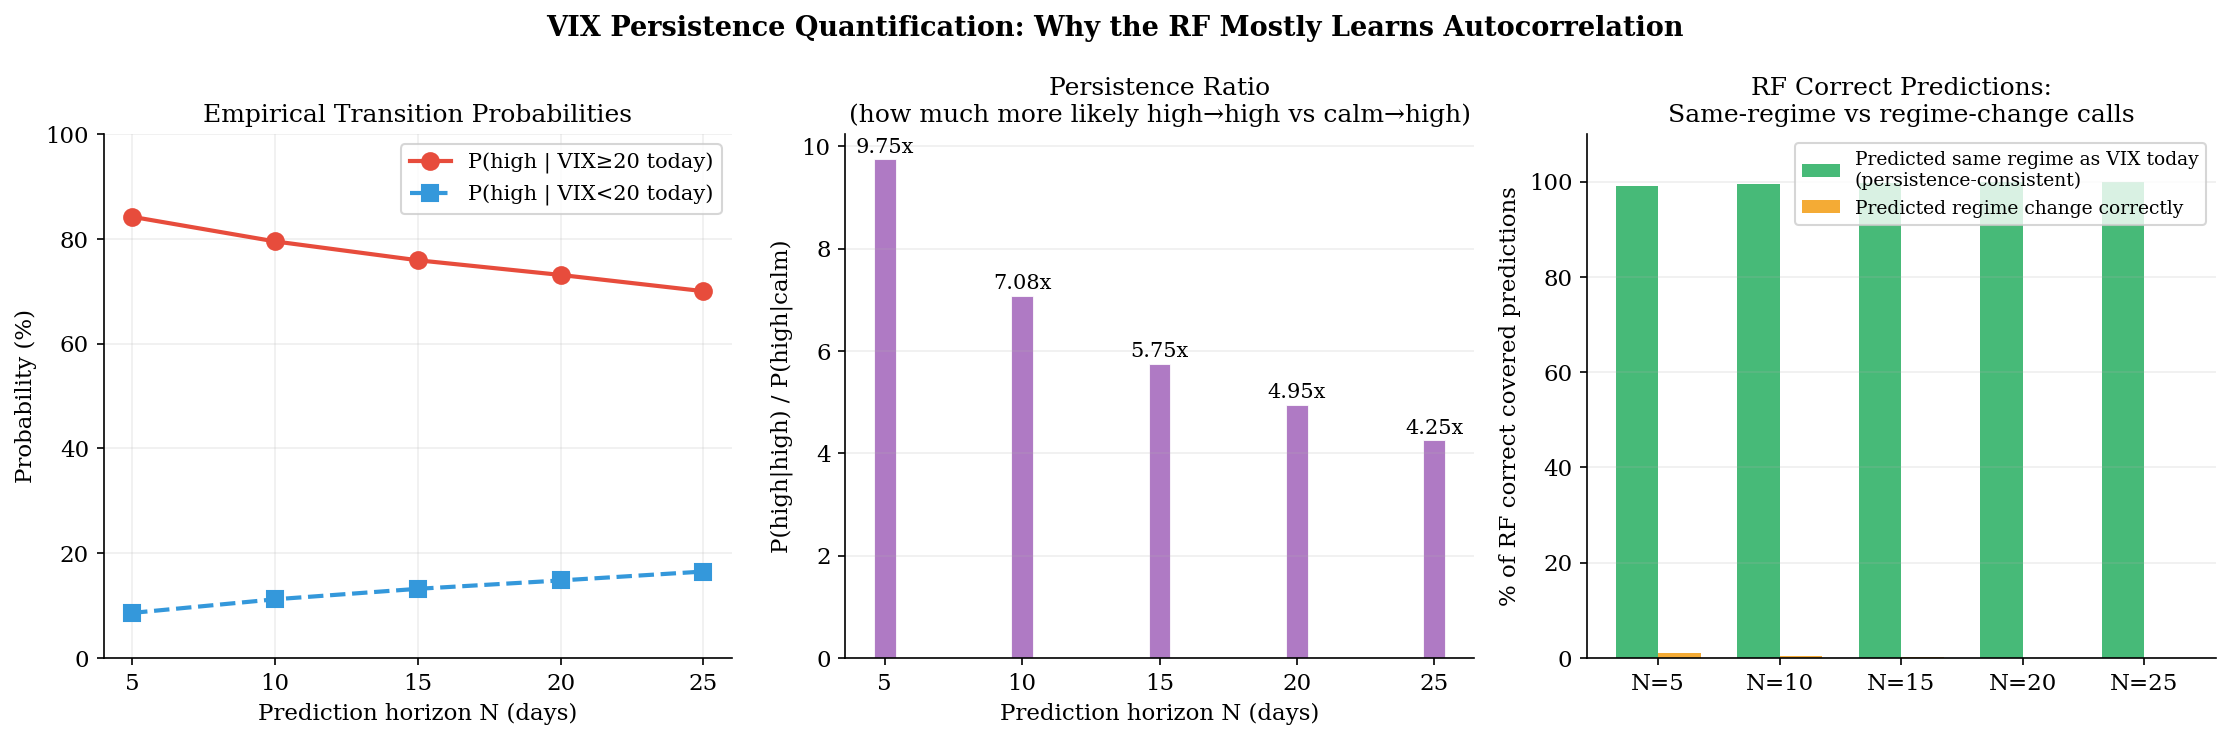
\includegraphics[width=\textwidth]{persistence_quantify.png}
    \caption{Left: empirical transition probabilities conditional on today's regime. Center:
    persistence ratio P(H$\mid$H)/P(H$\mid$C). Right: decomposition of RF correct covered
    predictions into same-regime and regime-change calls. At $N \geq 20$, 100\% of correct
    predictions are same-regime.}
    \label{fig:persist_quant}
\end{figure}

At $N = 5$, the probability of VIX being high in 5 days is 84.2\% given it is high today,
compared to only 8.6\% given it is calm today---a 9.8$\times$ ratio. On covered days, 99.0\%
of the RF's correct predictions at $N = 5$ are same-regime calls; at $N \geq 20$, every correct
covered prediction is a persistence call. The RF adds no directional forecasting beyond VIX
autocorrelation on the days it chooses to cover.

\subsection{Regime Transition Analysis}
\label{sec:transitions}

We classify each test day by the regime at time $t$ and the realized regime at $t + N$, creating
four transition categories: calm$\to$calm, calm$\to$high, high$\to$calm, and high$\to$high.

\begin{table}[H]
\centering
\caption{RF selective coverage and accuracy by regime transition type ($\tau = 0.25$, test set).
Calm$\to$high accuracy is \textbf{0\%} at all horizons: every covered prediction on a day about
to spike is a confident ``stay calm'' signal.}
\label{tab:trans}
\begin{tabular}{lcccccc}
\toprule
Transition & \multicolumn{3}{c}{$N = 5$} & \multicolumn{3}{c}{$N = 10$} \\
\cmidrule(lr){2-4}\cmidrule(lr){5-7}
           & Days & Coverage & Acc (covered) & Days & Coverage & Acc (covered) \\
\midrule
calm $\to$ calm & 614 & 87.1\% & 99.6\% & 587 & 71.6\% & 100.0\% \\
calm $\to$ high &  79 & 45.6\% & \textbf{0.0\%}   & 101 & 41.6\% & \textbf{0.0\%} \\
high $\to$ calm &  84 & 35.7\% & 23.3\%            & 111 & 18.0\% & 10.0\% \\
high $\to$ high & 222 & 72.5\% & 99.4\%            & 199 & 59.3\% & 100.0\% \\
\bottomrule
\end{tabular}
\end{table}

\begin{figure}[H]
    \centering
    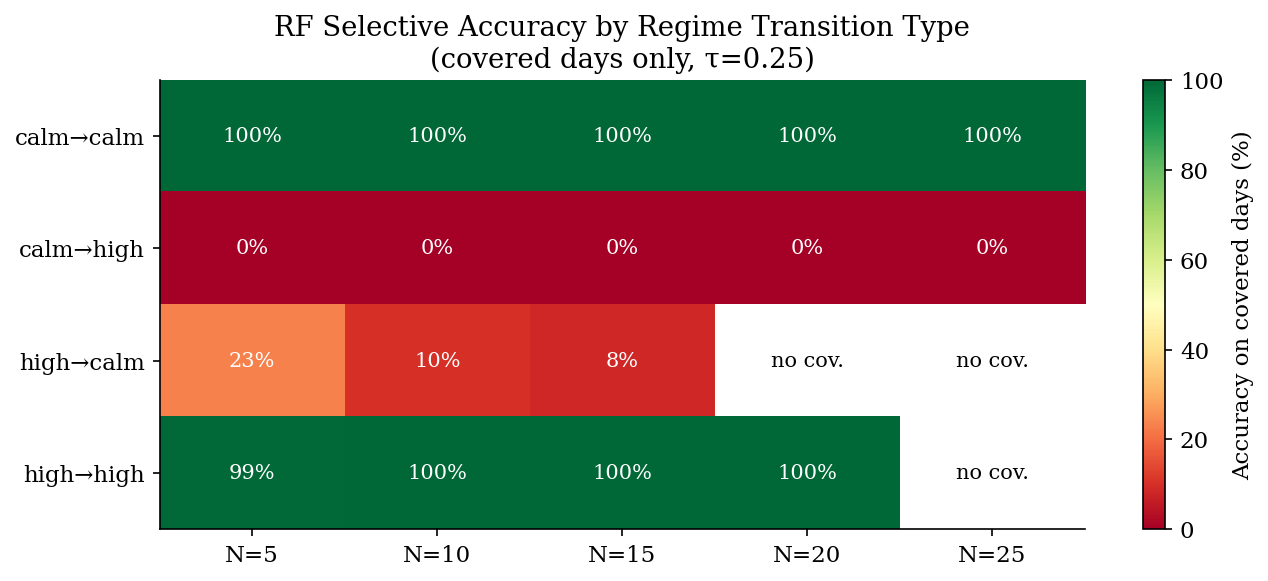
\includegraphics[width=0.65\textwidth]{transition_analysis.png}
    \caption{RF selective accuracy by regime transition type and horizon (covered days only,
    $\tau = 0.25$). Calm$\to$high rows are uniformly 0\% at all horizons.}
    \label{fig:trans}
\end{figure}

At $N = 5$, the model covers 36 of 79 calm$\to$high days (45.6\%). On every single one of those
36 days, it issues a confident ``stay calm'' prediction and is wrong. The mechanism is clear: VIX
comfortably below 20 generates calibrated probabilities below 0.25, triggering a high-confidence
calm prediction.

\paragraph{Structural caveat.}
This failure is not a model-specific defect: it is an expected structural property of the
prediction problem. Calm$\to$high transitions are disproportionately triggered by exogenous
events---geopolitical shocks, central bank surprises, sudden liquidity dislocations---whose onset
leaves no advance signature in publicly available daily price and macro features. The diagnostic
value of 0\% covered accuracy is that the confidence filter fails to surface its own ignorance,
issuing confident wrong predictions on covered transition days rather than abstaining.

\paragraph{Event case studies.}
Figure~\ref{fig:events} documents the model's behavior during four major volatility events in
the test set: the 2022 bear-market VIX peak (June 2022), the UK gilt crisis (October 2022), the
SVB banking collapse (March 2023), and the Japan carry-trade unwind (August 2024, when VIX
reached 65).

\begin{figure}[H]
    \centering
    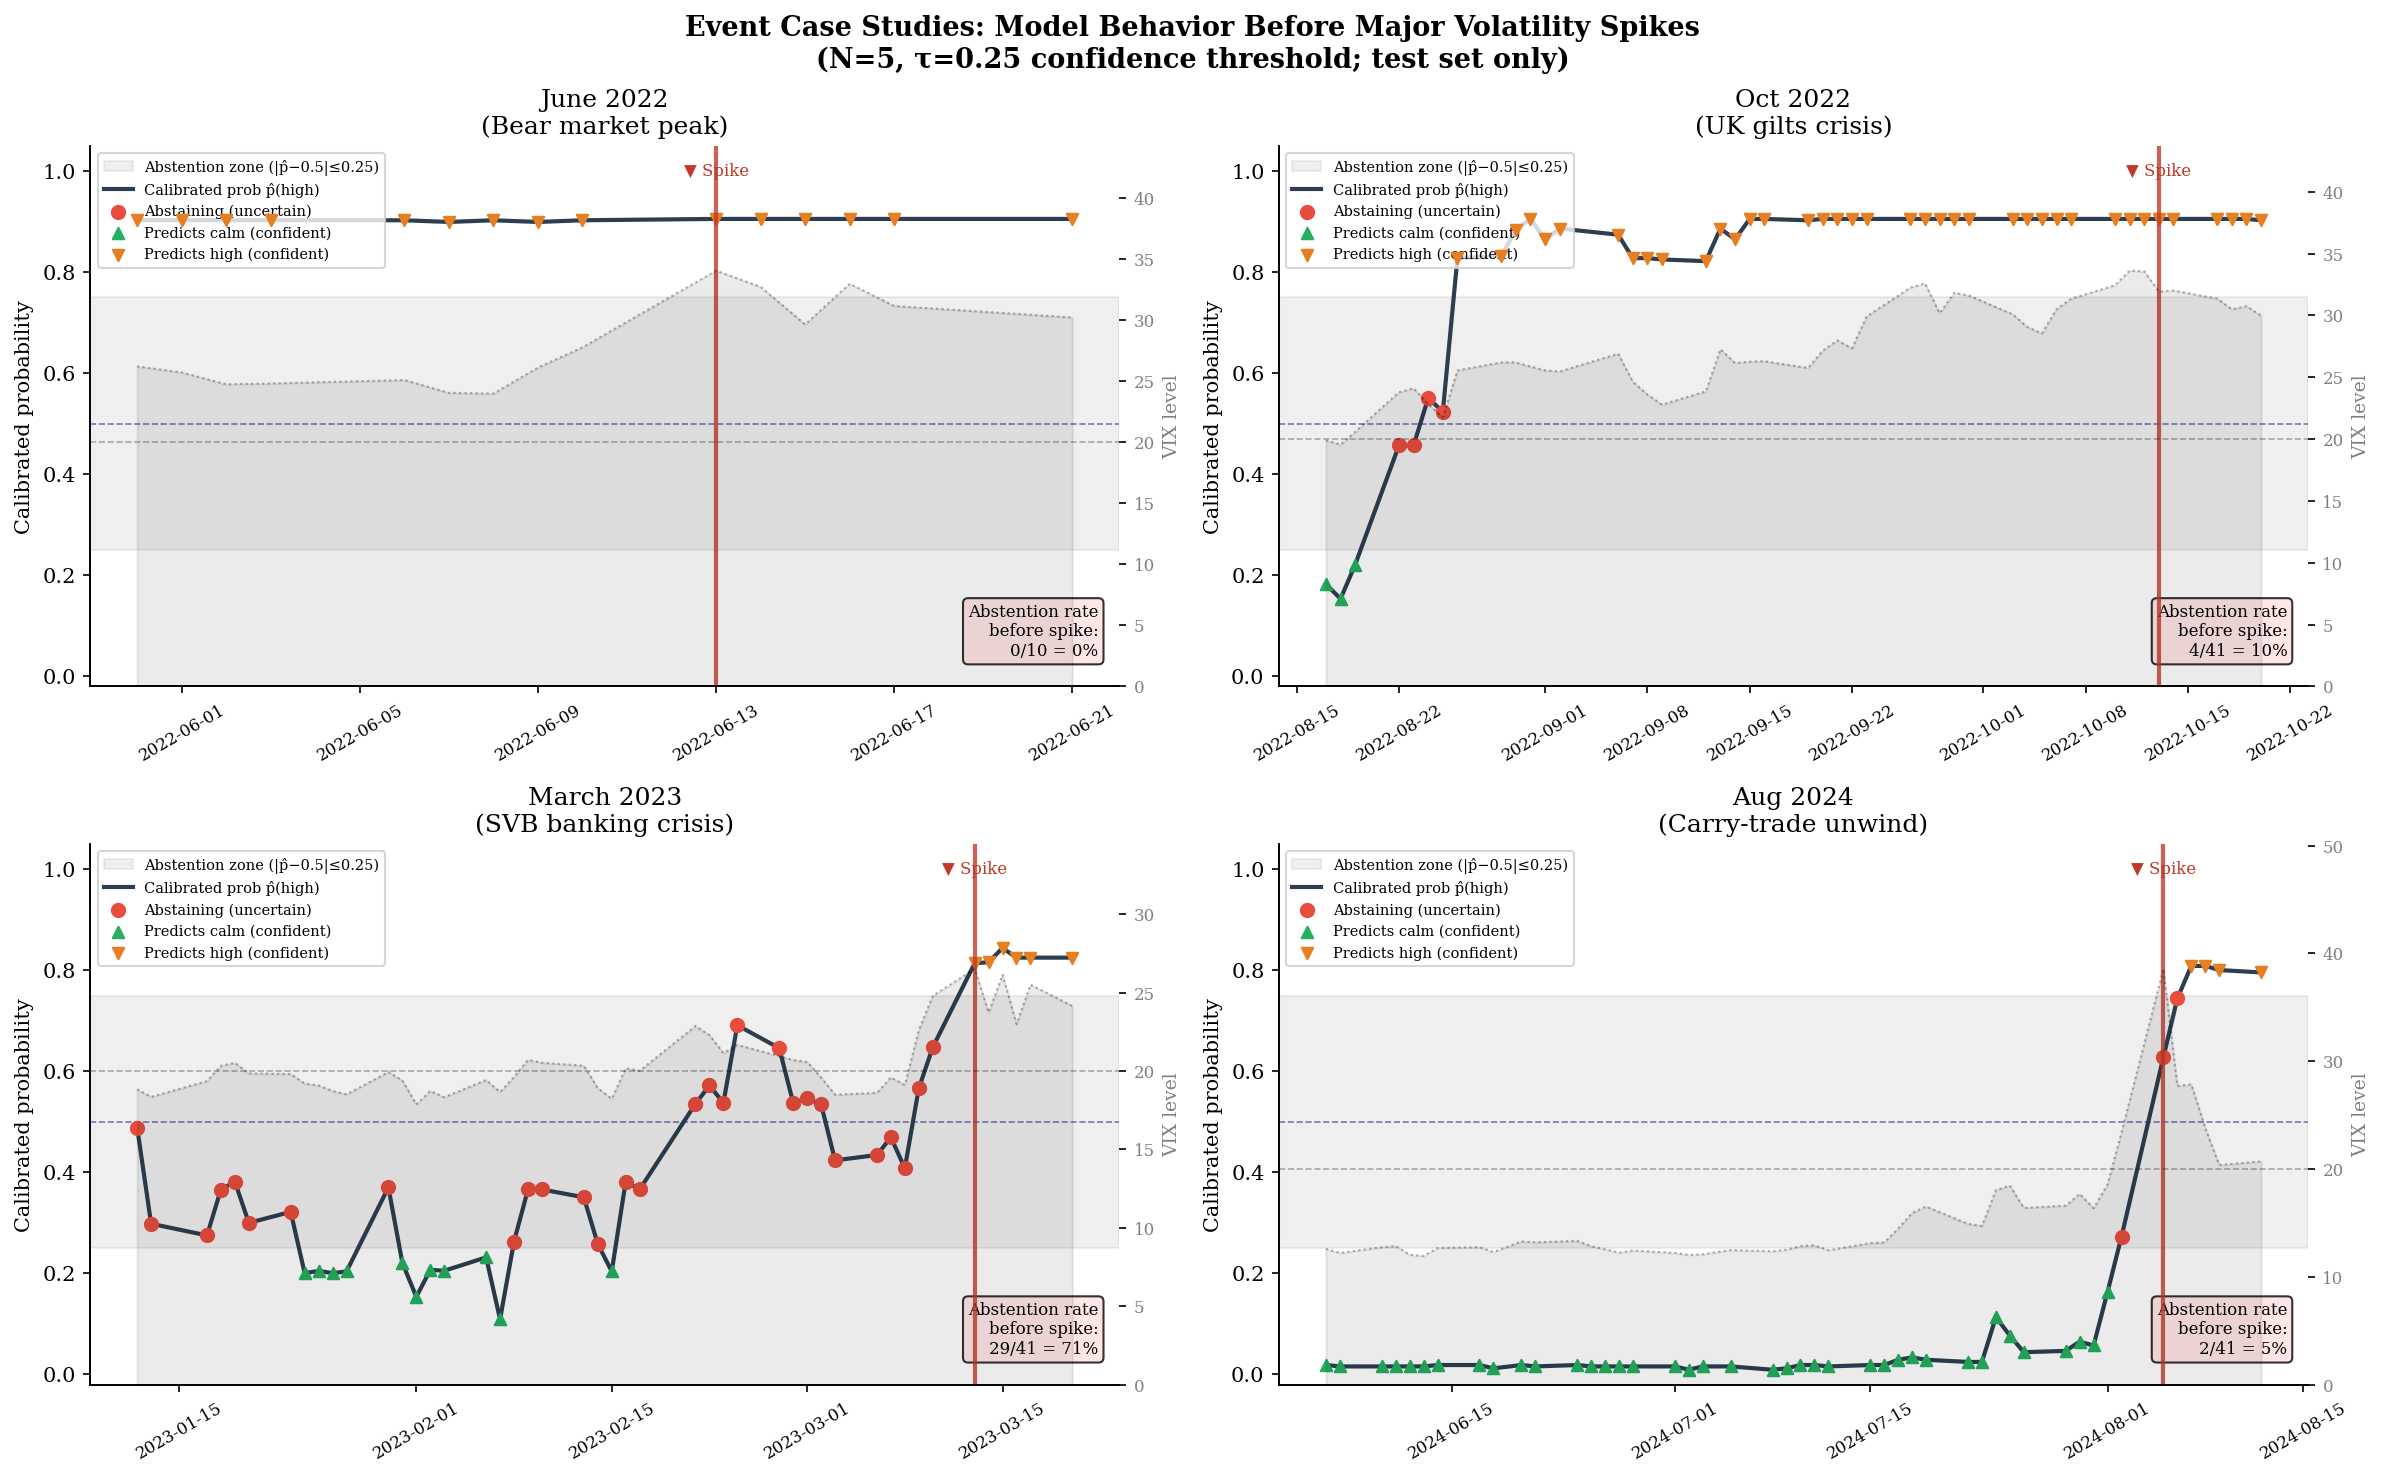
\includegraphics[width=\textwidth]{event_case_studies.png}
    \caption{Model behavior ($\hat{p}_t$, $N = 5$, $\tau = 0.25$) for 40 trading days before
    four major volatility events. In all four cases the model issues confident calm predictions
    leading up to the event.}
    \label{fig:events}
\end{figure}

Across all four events the pattern is consistent: the model issues confident ``stay calm''
predictions on the days leading up to each spike. The August 2024 carry-trade unwind shows
essentially no anticipatory signal; $\hat{p}_t$ remains below $0.5 - \tau$ until the day the
spike materializes.

\paragraph{Cost-weighting does not rescue calm$\to$high recall.}
To confirm the failure is informational rather than objective-function-driven, we refit the RF
with explicit class weights $\{0{:}1, 1{:}w\}$ for $w \in \{1, 5, 10, 20\}$.

\begin{table}[H]
\centering
\caption{Effect of class-weighting on transition coverage and selective accuracy. Calm$\to$high
accuracy is \textbf{0.0\%} at every weight for both horizons.}
\label{tab:reweight}
\begin{tabular}{ccrrcrc}
\toprule
$N$ & $w$ & C$\to$H Cov & C$\to$H Acc & C$\to$C Cov & C$\to$C Acc & Sel Acc \\
\midrule
5 &  1 & 45.6\% & \textbf{0.0\%} & 87.1\% & 99.6\%  & 91.9\% \\
5 &  5 & 46.8\% & \textbf{0.0\%} & 87.1\% & 100.0\% & 92.2\% \\
5 & 10 & 49.4\% & \textbf{0.0\%} & 87.3\% & 100.0\% & 92.3\% \\
5 & 20 & 48.1\% & \textbf{0.0\%} & 84.4\% & 100.0\% & 91.8\% \\
\midrule
10 &  1 & 41.6\% & \textbf{0.0\%} & 71.6\% & 100.0\% & 90.0\% \\
10 &  5 & 49.5\% & \textbf{0.0\%} & 77.7\% & 100.0\% & 89.5\% \\
10 & 10 & 58.4\% & \textbf{0.0\%} & 80.4\% & 100.0\% & 87.4\% \\
10 & 20 & 57.4\% & \textbf{0.0\%} & 82.8\% & 100.0\% & 87.4\% \\
\bottomrule
\end{tabular}
\end{table}

The failure to predict calm$\to$high transitions is \emph{informational}, not
objective-function-driven.

\paragraph{Abstention as a leading indicator.}

\begin{figure}[H]
    \centering
    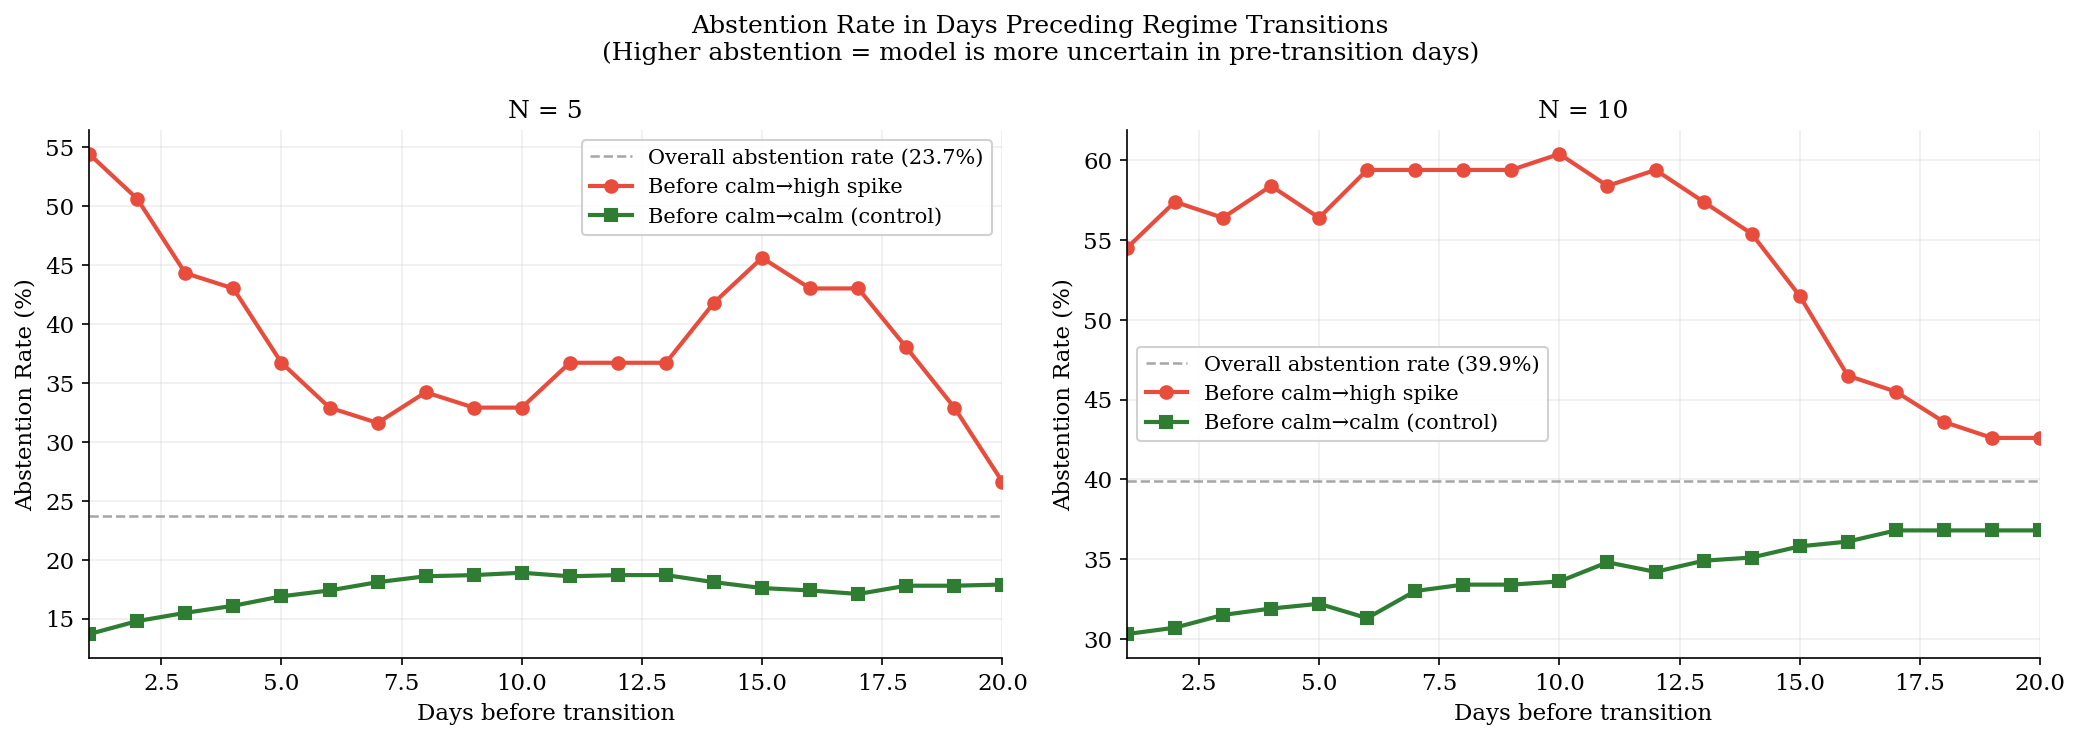
\includegraphics[width=0.85\textwidth]{abstention_analysis.png}
    \caption{Abstention rate before calm$\to$high transitions (red) vs.\ calm$\to$calm days
    (green). At lag = 1 day, the abstention rate before spikes is more than double the overall
    rate.}
    \label{fig:abstention}
\end{figure}

At $N = 5$, the abstention rate immediately before a calm$\to$high transition is 54.4\%,
compared to 13.7\% before calm$\to$calm days and 23.7\% overall---a 2.3$\times$ elevation.
However, a confound test shows that VIX proximity to the threshold (AUC $= 0.805$) explains most
of this signal; the abstention indicator alone achieves AUC $= 0.708$. At $N = 5$, abstention
carries a small residual signal beyond proximity (likelihood-ratio $p = 0.001$ on the evaluation
sample, treated as descriptive rather than confirmatory). This observation should be treated as
hypothesis-generating and requires dedicated out-of-sample confirmation.

\subsection{Walk-Forward Validation}
\label{sec:wf}

\begin{table}[H]
\centering
\caption{5-fold expanding walk-forward validation. Shaded rows indicate that at $N = 20$ the
RF/HGB standard deviations exceed 25 pp; persistence remains stable.}
\label{tab:wf}
\begin{tabular}{cccccc}
\toprule
Model & $N$ & Mean Baseline & Std & Mean Selective & Std \\
\midrule
Random Forest    & 5  & 82.8\% & 9.7\%  & 92.2\% & 1.7\%  \\
Persistence      & 5  & 88.0\% & 3.2\%  & \textbf{93.9\%} & 3.2\%  \\
HGB              & 5  & 84.0\% & 8.0\%  & 84.6\% & 9.7\%  \\
\midrule
Random Forest    & 10 & 72.3\% & 22.7\% & 85.9\% & 7.7\%  \\
Persistence      & 10 & 84.8\% & 4.5\%  & \textbf{91.3\%} & 4.1\%  \\
HGB              & 10 & 70.9\% & 22.9\% & 77.3\% & 15.2\% \\
\midrule
\rowcolor[gray]{0.9}
Random Forest    & 20 & 67.5\% & 22.8\% & 67.1\% & 28.3\% \\
Persistence      & 20 & 81.5\% & 3.9\%  & \textbf{86.2\%} & 7.7\%  \\
\rowcolor[gray]{0.9}
HGB              & 20 & 63.6\% & 25.2\% & 61.4\% & 29.9\% \\
\bottomrule
\end{tabular}
\end{table}

Coverage-matched persistence at $N = 5$ achieves 93.9\% $\pm$ 3.2\%---higher mean than RF
(92.2\% $\pm$ 1.7\%) with roughly double the fold-to-fold variance. At $N = 10$, persistence
(91.3\% $\pm$ 4.1\%) exceeds RF selective (85.9\% $\pm$ 7.7\%). At $N = 20$, both RF and HGB
show standard deviations exceeding 25 pp, while persistence remains stable. The practical
reliable prediction window is approximately $N \leq 10$.

\subsection{LSTM Comparison}
\label{sec:lstm}

A two-layer LSTM network is trained on sliding windows of the past 20 trading days of all 36
features, using the same 80/20 chronological split. The LSTM uses hidden size 64, dropout 0.3,
and is trained for 40 epochs with the Adam optimizer.

\begin{table}[H]
\centering
\caption{LSTM vs.\ RF at $\tau = 0.25$. BalAcc = balanced accuracy on covered days.}
\label{tab:lstm}
\begin{tabular}{cccccc}
\toprule
$N$ & LSTM Sel Acc & LSTM Cov & LSTM BalAcc & RF Sel Acc & RF Cov \\
\midrule
5  & 76.5\% & 87.0\% & 76.0\% & 91.7\% & 77.0\% \\
10 & 71.8\% & 90.7\% & 64.7\% & 89.3\% & 64.3\% \\
\bottomrule
\end{tabular}
\end{table}

The LSTM achieves non-zero calm$\to$high covered accuracy (34.9\% at $N = 5$; 19.1\% at
$N = 10$)---unlike the RF's 0\%---but both figures are substantially below the 50\% random
baseline, meaning the LSTM is wrong more often than right on transition days. Architectural
richness (20-day temporal memory) does not resolve the information constraint: the daily feature
set does not carry the event-anticipation content needed to forecast volatility spikes.

\subsection{SHAP Feature Attribution}
\label{sec:shap}

\begin{figure}[H]
    \centering
    
\includegraphics[width=0.92\textwidth]{shap_analysis.png}
    \caption{Mean absolute SHAP values (top 15 of 36 features) at $N = 5$ (left) and $N = 10$
    (right). VIX technical features account for 71.9\% and 64.7\% of total SHAP mass,
    respectively.}
    \label{fig:shap}
\end{figure}

VIX technical features account for \textbf{71.9\%} of total SHAP mass at $N = 5$ and
\textbf{64.7\%} at $N = 10$. The dominant features are all smoothed or envelope transforms of
the current VIX level. SHAP confirms that the model's predictions are driven overwhelmingly by
VIX autocorrelation, with negligible contribution from the broader cross-asset and macro feature
set.

\subsection{Statistical Significance of the Persistence Gap}
\label{sec:bootstrap}

We apply a moving-block bootstrap to the paired accuracy difference (RF selective minus
persistence, at matched coverage). Block length is set to $\max(\sqrt{N_\text{test}},\, 20)
\approx 32$ days \citep{kunsch1989}; 2,000 bootstrap replicates are drawn.

\begin{table}[H]
\centering
\caption{Moving-block bootstrap 95\% confidence intervals for the RF vs.\ persistence accuracy
gap. All CIs include 0; no gap is statistically significant at the 5\% level.}
\label{tab:boot}
\begin{tabular}{crrr}
\toprule
$N$ & Gap (pp) & 95\% CI lower & 95\% CI upper \\
\midrule
5  & $+0.30$ & $-2.26$ & $+2.80$ \\
10 & $+1.88$ & $-1.11$ & $+4.17$ \\
15 & $+2.07$ & $-3.03$ & $+7.70$ \\
20 & $+2.28$ & $-5.01$ & $+11.03$ \\
25 & $+6.52$ & $-2.86$ & $+18.87$ \\
\bottomrule
\end{tabular}
\end{table}

No gap is statistically significant at the 5\% level. The McNemar test sharpens this: at
$N \geq 10$, RF and persistence make \emph{identical} predictions on every jointly covered day
($b = c = 0$, $\chi^2 = 0$, $p = 1.000$). The Table~\ref{tab:boot} accuracy gaps are therefore
attributable entirely to differences in which days each rule covers, not to differing predictions
on shared days. Excluding the 2022 bear-market period (149--165 test days) leaves all qualitative
conclusions unchanged: calm$\to$high covered accuracy remains 0\% at all horizons.

\subsection{Cost-Weighted Utility Analysis}
\label{sec:utility}

\begin{equation}
    U = -\frac{\text{FP} + C \cdot \text{FN}}{n_{\text{predictions}}}
    \label{eq:utility}
\end{equation}

\begin{table}[H]
\centering
\caption{Cost-weighted utility per prediction under different FN/FP cost ratios $C$. Higher
utility (closer to 0) is better. Bolded entries show where persistence dominates RF selective.}
\label{tab:utility}
\begin{tabular}{ccrrrr}
\toprule
$N$ & $C$ & RF Selective & Persistence & RF Baseline & Always Calm \\
\midrule
5 &  1 & $-0.081$ & $-0.087$ & $-0.166$ & $-0.301$ \\
5 &  5 & $-0.276$ & $-0.286$ & $-0.515$ & $-1.507$ \\
5 & 10 & $-0.518$ & $-0.535$ & $-0.950$ & $-3.013$ \\
5 & 20 & $-1.004$ & $-1.033$ & $-1.821$ & $-6.026$ \\
\midrule
10 &  1 & $-0.100$ & $-0.120$ & $-0.205$ & $-0.301$ \\
10 &  5 & $-0.380$ & $\mathbf{-0.326}$ & $-0.626$ & $-1.503$ \\
10 & 10 & $-0.730$ & $\mathbf{-0.584}$ & $-1.152$ & $-3.006$ \\
10 & 20 & $-1.430$ & $\mathbf{-1.100}$ & $-2.204$ & $-6.012$ \\
\bottomrule
\end{tabular}
\end{table}

At $N = 10$, persistence at matched coverage dominates RF selective prediction under any moderate
false-negative cost asymmetry ($C \geq 5$). The RF selective framework is utility-beneficial only
when false positives are as costly as false negatives ($C = 1$).

% -----------------------------------------------------------------------
\section{Replication: S\&P 500 Trend-Regime Classification}
\label{sec:replication}
% -----------------------------------------------------------------------

To test whether the persistence illusion is specific to volatility forecasting, we replicate the
full diagnostic protocol on S\&P 500 trend-regime classification using the same feature set and
model specification. The label is:
\begin{equation}
    \text{BEAR}_{N,t} = \begin{cases} 1 & \text{if } \text{SP500}_{t+N} < \overline{\text{SP500}}_{200,t+N} \\ 0 & \text{otherwise} \end{cases}
\end{equation}

\begin{table}[H]
\centering
\caption{S\&P 500 trend-regime replication. RF$-$Persist is \emph{negative} at every horizon:
persistence strictly dominates the RF selective classifier.}
\label{tab:sp500}
\begin{tabular}{ccccccc}
\toprule
$N$ & Base rate & Coverage & Persistence & HAR-analog & RF Sel & RF$-$Persist \\
\midrule
5  & 22.0\% & 74.4\% & \textbf{100.0\%} & 86.9\% & 96.0\% & $-4.0$ pp \\
10 & 21.9\% & 68.3\% & \textbf{99.6\%}  & 86.4\% & 94.9\% & $-4.7$ pp \\
15 & 21.9\% & 69.7\% & \textbf{97.3\%}  & 86.7\% & 90.9\% & $-6.3$ pp \\
20 & 21.8\% & 70.3\% & \textbf{94.9\%}  & 84.9\% & 87.7\% & $-7.1$ pp \\
25 & 21.7\% & 59.5\% & \textbf{94.8\%}  & 84.8\% & 88.3\% & $-6.4$ pp \\
\bottomrule
\end{tabular}
\end{table}

\begin{table}[H]
\centering
\caption{S\&P 500 transition accuracy. Bull$\to$bear covered accuracy is \textbf{0\%}---exact
mirror of VIX calm$\to$high.}
\label{tab:sp500_trans}
\begin{tabular}{cccccc}
\toprule
$N$ & Transition & Days & Coverage & Acc (covered) & Same-regime \% \\
\midrule
5  & bull$\to$bull &  749 & 88.8\% & 100.0\% & 99.2\% \\
5  & bull$\to$bear &   25 & 68.0\% & \textbf{0.0\%} & \\
\midrule
10 & bull$\to$bull &  730 & 86.2\% & 100.0\% & 98.6\% \\
10 & bull$\to$bear &   39 & 71.8\% & \textbf{0.0\%} & \\
\bottomrule
\end{tabular}
\end{table}

\begin{figure}[H]
    \centering
    
\includegraphics[width=\textwidth]{sp500_replication.png}
    \caption{S\&P 500 trend-regime replication. Left: RF vs.\ persistence---persistence dominates
    at all horizons. Center: persistence ratio of 23.8$\times$ at $N = 5$. Right: bull$\to$bear
    covered accuracy is 0\%, replicating the VIX calm$\to$high finding.}
    \label{fig:sp500}
\end{figure}

The persistence ratio is \textbf{23.8$\times$} at $N = 5$---more than twice the VIX ratio of
9.7$\times$---and persistence beats the RF at \emph{every horizon} (RF$-$Persist: $-4.0$ to
$-7.1$ pp). Bull$\to$bear covered accuracy is \textbf{0.0\%} at both $N = 5$ and $N = 10$,
replicating the VIX calm$\to$high finding exactly. The replication establishes that the
persistence illusion is a structural consequence of applying selective prediction to any
autocorrelated binary time series, not a VIX-specific artifact.

% -----------------------------------------------------------------------
\section{Conclusions}
\label{sec:conclusion}
% -----------------------------------------------------------------------

This paper applies a six-component diagnostic protocol to VIX regime classification and shows
that headline selective prediction accuracy reflects autocorrelation, not machine learning skill.
The confidence filter achieves 0\% accuracy on every calm$\to$high transition it covers; explicit
cost-weighting up to $20{\times}$ does not rescue this. A McNemar test on jointly covered days
finds $b = c = 0$ at $N \geq 10$: RF and persistence make identical predictions on every shared
day, so the accuracy gap is entirely composition-driven. Three-feature HAR logistic regression
matches or exceeds 36-feature RF in point estimate at four of five horizons; cost-weighted utility
at $N = 10$ favors persistence whenever false negatives are more costly than false alarms.

SHAP attribution shows VIX technical features account for 71.9\% of model prediction mass; a
two-layer LSTM also fails on calm$\to$high transitions (19--35\% accuracy, below random chance);
and the full diagnostic replicates on S\&P 500 trend regimes with bull$\to$bear covered accuracy
of 0\%.

\subsection*{Limitations}

The feature set consists of publicly available daily market data. Calm$\to$high transitions are
disproportionately triggered by exogenous shocks---geopolitical events, policy surprises, sudden
liquidity crises---that leave no advance signature in daily price features. The four-year test
period ($\approx$1,000 trading days) is underpowered for distinguishing accuracy differences of
1--3 pp under serial dependence.

\subsection*{Future Work}

The primary open direction is feature enrichment: incorporating event-anticipation content such
as options skew dynamics, credit spreads, or order-flow imbalance. A two-stage system using the
abstention rate as a leading indicator followed by a conditional spike-prediction model is a
second natural direction. Third, the diagnostic protocol should be applied to additional
autocorrelated regime classification tasks---credit spread regimes, recession prediction,
currency crisis indicators---to characterize how the persistence ratio relates to the severity
of the selective-prediction bias.

% -----------------------------------------------------------------------
% REQUIRED STATEMENTS
% -----------------------------------------------------------------------

\section*{Author Contributions}

Conceptualization, A.G.; methodology, A.G.; software, A.G.; formal analysis, A.G.; data
curation, A.G.; investigation, A.G.; writing---original draft, A.G.; writing---review and
editing, J.L.; visualization, A.G.; supervision, J.L. All authors have read and agreed to the
published version of the manuscript.

\section*{Funding}

This research received no external funding.

\section*{Data Availability Statement}

The data used in this study are publicly available. VIX, VIX3M, S\&P 500, gold, Treasury yield,
DXY, and SKEW data are available from Yahoo Finance (\url{https://finance.yahoo.com}).
Macroeconomic data (Federal Funds Rate and yield curve spread) are available from the Federal
Reserve Economic Data (FRED) API (\url{https://fred.stlouisfed.org}).

\section*{Conflicts of Interest}

The authors declare no conflicts of interest.

\section*{Declaration of Generative AI Use}

During the preparation of this work, the authors used Claude (Anthropic) to critique earlier
manuscript drafts and improve writing clarity. The authors reviewed and edited the output as
needed and take full responsibility for the content of the published article.

% -----------------------------------------------------------------------
\appendix
\section{Complete Feature List}
\label{app:features}

\begin{table}[H]
\centering
\caption{All 36 engineered features, grouped by category. All features are computed from
information available at or before prediction date $t$.}
\label{tab:features}
\small
\resizebox{\textwidth}{!}{%
\begin{tabular}{llll}
\toprule
\# & Feature name & Definition & Category \\
\midrule
1  & VIX\_SMA10        & 10-day simple moving average of VIX                        & VIX trend \\
2  & VIX\_SMA20        & 20-day simple moving average of VIX                        & VIX trend \\
3  & VIX\_MOM10        & VIX$_t$ $-$ VIX$_{t-10}$                                  & VIX momentum \\
4  & VIX\_MOM20        & VIX$_t$ $-$ VIX$_{t-20}$                                  & VIX momentum \\
5  & VIX\_ROC10        & $({\rm VIX}_t / {\rm VIX}_{t-10}) - 1$                     & VIX momentum \\
6  & VIX\_ROC20        & $({\rm VIX}_t / {\rm VIX}_{t-20}) - 1$                     & VIX momentum \\
7  & VIX\_BB\_STD      & 20-day rolling std.\ of VIX                                & VIX Bollinger \\
8  & VIX\_BB\_UPPER    & VIX\_SMA20 $+$ 2$\times$VIX\_BB\_STD                       & VIX Bollinger \\
9  & VIX\_BB\_LOWER    & VIX\_SMA20 $-$ 2$\times$VIX\_BB\_STD                       & VIX Bollinger \\
10 & VIX\_BB\_POSITION & (VIX$_t$ $-$ VIX\_BB\_LOWER) / (4$\times$VIX\_BB\_STD)    & VIX Bollinger \\
11 & VIX\_RSI14        & 14-day Relative Strength Index of VIX                      & VIX oscillator \\
12 & VIX\_MACROSS      & VIX\_SMA10 $-$ VIX\_SMA20                                  & VIX trend \\
13 & VIX\_TERM\_SPREAD & VIX3M$_t$ $-$ VIX$_t$                                      & VIX structure \\
\midrule
14 & SKEW\_LEVEL       & Raw CBOE SKEW index value                                  & Tail risk \\
15 & SKEW\_CHG5        & SKEW$_t$ $-$ SKEW$_{t-5}$                                  & Tail risk \\
16 & SKEW\_CHG20       & SKEW$_t$ $-$ SKEW$_{t-20}$                                 & Tail risk \\
\midrule
17 & SP500\_RET1       & Log return of S\&P 500 over 1 day                          & Equity \\
18 & SP500\_RET5       & Log return of S\&P 500 over 5 days                         & Equity \\
19 & SP500\_RET20      & Log return of S\&P 500 over 20 days                        & Equity \\
20 & SP500\_MOM10      & S\&P 500 price at $t$ $-$ price at $t-10$                  & Equity \\
21 & SP500\_MOM20      & S\&P 500 price at $t$ $-$ price at $t-20$                  & Equity \\
22 & SP500\_RVOL       & 20-day realized volatility of S\&P 500 daily returns        & Equity \\
23 & SP500\_DRAWDOWN   & 252-day maximum drawdown of S\&P 500                       & Equity \\
\midrule
24 & GOLD\_RET1        & Log return of gold futures over 1 day                      & Cross-asset \\
25 & GOLD\_RET5        & Log return of gold futures over 5 days                     & Cross-asset \\
26 & GOLD\_RET20       & Log return of gold futures over 20 days                    & Cross-asset \\
27 & TNY\_CHG1         & 10Y Treasury yield change over 1 day                       & Cross-asset \\
28 & TNY\_CHG5         & 10Y Treasury yield change over 5 days                      & Cross-asset \\
29 & TNY\_CHG20        & 10Y Treasury yield change over 20 days                     & Cross-asset \\
30 & DXY\_RET1         & Log return of DXY over 1 day                               & Cross-asset \\
31 & DXY\_RET5         & Log return of DXY over 5 days                              & Cross-asset \\
32 & DXY\_RET20        & Log return of DXY over 20 days                             & Cross-asset \\
\midrule
33 & FEDFUNDS\_CHG1M   & Federal Funds Rate change over $\approx$21 trading days    & Macro \\
34 & FEDFUNDS\_CHG3M   & Federal Funds Rate change over $\approx$63 trading days    & Macro \\
35 & YIELD\_CURVE\_CHG1M & T10Y2Y spread change over $\approx$21 trading days      & Macro \\
36 & YIELD\_CURVE\_CHG3M & T10Y2Y spread change over $\approx$63 trading days      & Macro \\
\bottomrule
\end{tabular}}
\end{table}

% -----------------------------------------------------------------------
\bibliographystyle{plainnat}
\begin{thebibliography}{99}

\bibitem[Bartlett and Wegkamp(2008)]{bartlett2008}
Bartlett, P.L.; Wegkamp, M.H.
Classification with a reject option using a hinge loss.
\textit{J. Mach. Learn. Res.} \textbf{2008}, \textit{9}, 1823--1840.

\bibitem[Bollerslev(1986)]{bollerslev1986}
Bollerslev, T.
Generalized autoregressive conditional heteroskedasticity.
\textit{J. Econom.} \textbf{1986}, \textit{31}, 307--327.

\bibitem[Breiman(2001)]{breiman2001}
Breiman, L.
Random forests.
\textit{Mach. Learn.} \textbf{2001}, \textit{45}, 5--32.

\bibitem[Chen and Guestrin(2016)]{chen2016}
Chen, T.; Guestrin, C.
XGBoost: A scalable tree boosting system.
In \textit{Proceedings of the 22nd ACM SIGKDD International Conference on Knowledge Discovery
and Data Mining}; ACM: New York, NY, USA, 2016; pp. 785--794.

\bibitem[Chow(1970)]{chow1970}
Chow, C.K.
On optimum recognition error and reject tradeoff.
\textit{IEEE Trans. Inf. Theory} \textbf{1970}, \textit{16}, 41--46.

\bibitem[Corsi(2009)]{corsi2009}
Corsi, F.
A simple approximate long-memory model of realized volatility.
\textit{J. Financ. Econom.} \textbf{2009}, \textit{7}, 174--196.

\bibitem[Fernandes et al.(2014)]{fernandes2014}
Fernandes, M.; Medeiros, M.C.; Scharth, M.
Modeling and predicting the CBOE market volatility index.
\textit{J. Bank. Financ.} \textbf{2014}, \textit{40}, 1--10.

\bibitem[Geifman and El-Yaniv(2017)]{geifman2017}
Geifman, Y.; El-Yaniv, R.
Selective classification for deep neural networks.
\textit{Adv. Neural Inf. Process. Syst.} \textbf{2017}, \textit{30}.

\bibitem[Guidolin and Timmermann(2007)]{guidolin2007}
Guidolin, M.; Timmermann, A.
Asset allocation under multivariate regime switching.
\textit{J. Econ. Dyn. Control} \textbf{2007}, \textit{31}, 3503--3544.

\bibitem[Hamilton(1989)]{hamilton1989}
Hamilton, J.D.
A new approach to the economic analysis of nonstationary time series and the business cycle.
\textit{Econometrica} \textbf{1989}, \textit{57}, 357--384.

\bibitem[Kunsch(1989)]{kunsch1989}
Kunsch, H.R.
The jackknife and the bootstrap for general stationary observations.
\textit{Ann. Stat.} \textbf{1989}, \textit{17}, 1217--1241.

\bibitem[Lundberg and Lee(2017)]{lundberg2017}
Lundberg, S.M.; Lee, S.I.
A unified approach to interpreting model predictions.
\textit{Adv. Neural Inf. Process. Syst.} \textbf{2017}, \textit{30}.

\bibitem[Whaley(2009)]{whaley2009}
Whaley, R.E.
Understanding the VIX.
\textit{J. Portf. Manag.} \textbf{2009}, \textit{35}, 98--105.

\end{thebibliography}

\end{document}
